\documentclass[letterpaper]{article}
\usepackage[square,sort,comma,numbers]{natbib}
\newcommand{\citeasnoun}[1]{Ref.~\citenum{#1}}

../../../../tex/scufftex.tex

\newcommand\supsstar[1]{^{\hbox{\scriptsize{#1}}*}}
\newcommand\suptstar[1]{^{\hbox{\scriptsize{#1}}*}}
\newcommand{\IF}{^{i\text{\scriptsize F}}}
\newcommand{\IFFlux}{^{i\text{\tiny FFLUX}}}
\newcommand{\IT}{^{i\text{\scriptsize T}}}
\newcommand{\ITFlux}{^{i\text{\tiny TFLUX}}}
\newcommand{\PS}{^{\text{\scriptsize P}\mc S}}
\newcommand{\IFS}{^{i\text{\scriptsize F}\mc S}}
\newcommand{\ITS}{^{i\text{\scriptsize T}\mc S}}
\newcommand{\wh}{\widehat}
%\newcommand{\vbchi}{\boldsymbol{\chi}}

\graphicspath{{figures/}}

%------------------------------------------------------------
%------------------------------------------------------------
%- Special commands for this document -----------------------
%------------------------------------------------------------
%------------------------------------------------------------

%------------------------------------------------------------
%------------------------------------------------------------
%- Document header  -----------------------------------------
%------------------------------------------------------------
%------------------------------------------------------------
\title {{\sc scuff-neq} Technical Reference}
\author {Homer Reid}
\date {July 6, 2014}

%------------------------------------------------------------
%------------------------------------------------------------
%- Start of actual document
%------------------------------------------------------------
%------------------------------------------------------------

\begin{document}
\pagestyle{myheadings}
\markright{Homer Reid: {\sc scuff-neq} Technical Reference}
\maketitle

\tableofcontents

%%%%%%%%%%%%%%%%%%%%%%%%%%%%%%%%%%%%%%%%%%%%%%%%%%%%%%%%%%%%%%%%%%%%%%
%%%%%%%%%%%%%%%%%%%%%%%%%%%%%%%%%%%%%%%%%%%%%%%%%%%%%%%%%%%%%%%%%%%%%%
%%%%%%%%%%%%%%%%%%%%%%%%%%%%%%%%%%%%%%%%%%%%%%%%%%%%%%%%%%%%%%%%%%%%%%
\newpage
\section{Theoretical background}

{\sc scuff-neq} implements the ``fluctuating-surface-current''
(FSC) approach to computational fluctuation physics. The 
FSC method was originally developed for equilibrium Casimir
computations~\cite{Reid2009, Reid2011, Reid2013B} and later
extended to non-equilibrium phenomena in 
Refs.~\citenum{Rodriguez2012C} and \citenum{Rodriguez2013B}.
Here we present a quick summary of the key equations in this
approach; slightly more detail may be found in the Appendices.

%%%%%%%%%%%%%%%%%%%%%%%%%%%%%%%%%%%%%%%%%%%%%%%%%%%%%%%%%%%%%%%%%%%%%%
%%%%%%%%%%%%%%%%%%%%%%%%%%%%%%%%%%%%%%%%%%%%%%%%%%%%%%%%%%%%%%%%%%%%%%
%%%%%%%%%%%%%%%%%%%%%%%%%%%%%%%%%%%%%%%%%%%%%%%%%%%%%%%%%%%%%%%%%%%%%%
\subsection{Time-average quantities from surface-current bilinears}
\label{PQsFromSCBsSection}

The FSC approach begins with the observation that, in a
classical, deterministic frequency-domain scattering problem 
involving the fields of known time-harmonic external sources 
impinging upon a collection of material bodies, the time-average
values of many physical quantities of interest may be expressed 
as bilinear (quadratic) products of the \textit{surface currents} 
induced on the body surfaces by
the external fields. The quantities whose time-average values
may be be expressed in this way include both \textbf{(a)} 
spatially-resolved fluxes of energy and momentum at individual 
points in space, and \textbf{(b)} total (spatially-integrated) 
power-transfer rates, forces, and torques on individual bodies.

More specifically, let the six-vector of surface electric
and magnetic currents (flowing on the surfaces of \textit{all}
bodies in a geometry) be
%====================================================================%
\numeq{BigCDef}
{
  \bmc C(\vb x)\equiv{\vb K(\vb x) \choose \vb N(\vb x)}
  \approx \sum_{\alpha} c_\alpha \bmc B_\alpha(\vb x)
}
%====================================================================%
where we have discretized by approximating $\bmc C(\vb x)$ as an
expansion in a discrete set of six-vector basis
functions\footnote{In {\sc scuff-neq} these take the form
$\bmc B_\alpha=$ 
$\vb b_\alpha \choose 0$ 
or 
$0 \choose \vb b_\alpha$
where $\vb b_\alpha$ is a three-vector RWG basis function.
However, the FSC formalism is not specific to this choice.}
\{$\bmc B_\alpha(\vb x)$\}; here $\{c_\alpha\}$ are 
scalar expansion coefficients\footnote{In {\sc scuff-em} 
the basis functions are dimensionless and the expansion
coefficients have units of 
%====================================================================%
\begin{align*}
 \big[c_{2\alpha}\big]&=\frac{\text{Amperes}}{\text{meters}}
 \quad \text{(electric surface currents)}, \qquad
 \big[c_{2\alpha+1}\big]=\frac{\text{Volts}}{\text{meters}}
 \quad \text{(magnetic surface currents).}
\end{align*}} typically obtained by 
%====================================================================%
inverting a linear system to solve a scattering 
problem.
(We work at a fixed frequency $\omega$ and assume all fields
and currents vary in time like $e^{-i\omega t}$.)

Then the time-average values of physical quantities associated 
with power, force and torque (PFT)---including both spatially-resolved
PFT fluxes at individual points in space as well as spatially-integrated
quantities representing the total PFT on compact bodies---may 
generally be expressed as vector-matrix-vector products of the 
form
%====================================================================%
\numeq{QcQc} {Q = \vb c^\dagger \vb Q \vb c}
%====================================================================%
where $Q$ is the quantity of interest, $\vb c$ is the 
vector of surface-current coefficients in (\ref{BigCDef}),
and $\vb Q$ is a matrix
that depends on the quantity we are computing and the method we
use to compute it.

\paragraph{Spatially-resolved PFT fluxes} 
For example, the time-average Poynting vector and Maxwell stress 
tensor at a point $\vb x$---that is, the time-average fluxes,
in the $\vbhat{n}$ direction, of energy, of $\vbhat{u}$-directed
linear momentum, and of $\vbhat{u}$-directed angular momentum---are
given by
%====================================================================%
$$\begin{array}{*3{>{\displaystyle}l}}
\text{Energy flux: } \qquad 
&\vb P(\vb x) \cdot \vbhat{n} 
&=\frac{1}{2}\text{Re }
   \vb c^\dagger \vb Q\supt{PFLUX}(\vb x; \vbhat{n}) \vb c
\\[10pt]
\text{Linear momentum flux: } \qquad 
&\vbhat{u} \cdot \vb T(\vb x) \cdot \vbhat{n}
&=\frac{1}{2}\text{Re }
   \vb c^\dagger \vb Q\supt{FFLUX}(\vb x; \vbhat{u}, \vbhat{n}) \vb c
\\[10pt]
\text{Angular momentum flux: } \qquad 
&\vbhat{u} \cdot \Big[(\vb x-\vb x_0) \times \vb T(\vb x)\Big] \cdot \vbhat{n}
&=\frac{1}{2}\text{Re }
   \vb c^\dagger \vb Q\supt{TFLUX}(\vb x; \vb x_0, \vbhat{u}, \vbhat{n}) \vb c
\end{array}$$
%====================================================================%
where the form of the $\vb Q\supt{FLUX}$ matrices is derived in
an Appendix. (In the last line, $\vb x_0$ is the origin about which 
we are computing the torque).

\paragraph{Spatially-integrated PFT fluxes} 
On the other hand, the \textit{total} (spatially-integrated)
power absorbed by, and the $\vbhat{u}$-directed force and torque 
exerted on, one or more compact bodies contained within a 
closed bounding surface $\mc S$ are given by 
%====================================================================%
$$\begin{array}{*3{>{\displaystyle}l}}
\text{Absorbed power:} \qquad 
& P\sups{abs}
&=\frac{1}{2}\text{Re }
   \vb c^\dagger \vb Q\supt{PTOT}(\mc S) \vb c
\\[10pt]
\text{Force: } \qquad 
&\vbhat{u} \cdot \vb F
&=\frac{1}{2}\text{Re }
   \vb c^\dagger \vb Q\supt{FTOT}(\mc S; \vbhat{u}) \vb c
\\[10pt]
\text{Torque: } \qquad 
&\vbhat{u} \cdot \bmc T
&=\frac{1}{2}\text{Re }
   \vb c^\dagger \vb Q\supt{TTOT}(\mc S; \vb x_0, \vbhat{u}) \vb c
\end{array}$$
%====================================================================%
Explicit expressions for the $\vb Q\supt{TOT}$ matrices are given
in the Appendices.

%%%%%%%%%%%%%%%%%%%%%%%%%%%%%%%%%%%%%%%%%%%%%%%%%%%%%%%%%%%%%%%%%%%%%%
%%%%%%%%%%%%%%%%%%%%%%%%%%%%%%%%%%%%%%%%%%%%%%%%%%%%%%%%%%%%%%%%%%%%%%
%%%%%%%%%%%%%%%%%%%%%%%%%%%%%%%%%%%%%%%%%%%%%%%%%%%%%%%%%%%%%%%%%%%%%%
\subsection{Statistical averages of surface-current bilinears}

Equation (\ref{QcQc}) gives the time-average value of
a PFT quantity in a classical, deterministic scattering 
problem in which the surface currents $\vb c_\alpha$ are known.
The heart of the FSC approach to nonequilibrium phenomena 
is a concise formula for the \textit{statistical average} 
of such surface-current bilinears,
where the averaging is performed over thermal and quantum-mechanical
fluctuations of sources inside material bodies at fixed temperatures.
A precise statement of the FSC equivalence is as follows.

%%%%%%%%%%%%%%%%%%%%%%%%%%%%%%%%%%%%%%%%%%%%%%%%%%%%%%%%%%%%%%%%%%%%%%
\begin{itemize}

\item
If $Q$ is a physical quantity whose time-average
value (in a classical, deterministic scattering problem
involving time-harmonic fields at frequency $\omega$)
may be expressed as a bilinear function of the surface currents
with a matrix $\vb Q(\omega)$, i.e
%====================================================================%
\begin{subequations}
\begin{equation}
 \text{if} \qquad Q=\vb c^\dagger \vb Q \vb c
\end{equation}
%====================================================================%

\item
then the statistical \textit{average} of the quantity $Q$---where
the averaging is over quantum and thermal fluctuations---is given by
a sum over the contributions of fluctuating sources in all regions
of space:
%--------------------------------------------------------------------%
\begin{equation}
 \text{then} \qquad \big\langle Q\big\rangle
  = \int_0^\infty \, \sum_r \, \Theta(T_r,\omega) \Phi_r(\omega)\,d\omega 
\end{equation}
where 
$\Theta(T_r,\omega) = \frac{\hbar\omega}{e^{\hbar \omega/kT_r} - 1}$
is the Bose-Einstein factor for the temperature $T_r$ of 
region $r$, and where the ``generalized flux'' $\Phi_r$
is the trace of a four-matrix product involving the $\vb Q$ matrix:
%====================================================================%
\begin{equation}
\Phi_s
  = \frac{2}{\pi} 
    \Tr\left\{ \vb Q 
               \underbrace{\vb W \overline{\vb G}_r \vb W^\dagger}
                         _{\vb R_s}
       \right\}.
\end{equation}
%====================================================================%
\label{FSCEquivalence}%
\end{subequations}
%--------------------------------------------------------------------%
Here $\vb W$ is the inverse of the BEM matrix for the 
\textit{entire} collection of bodies and $\overline{\vb G}_r$ 
is a symmetrized version of a portion of the BEM matrix for region
$r$ alone.

\end{itemize}
%%%%%%%%%%%%%%%%%%%%%%%%%%%%%%%%%%%%%%%%%%%%%%%%%%%%%%%%%%%%%%%%%%%%%
The matrix $\vb R_s$ in (\ref{FSCEquivalence})---the ``Rytov''
matrix---furnishes a concise description of the fluctuating sources
inside body $s$. For a given output quantity 
$Q$, the generalized flux $\Phi_s$ is the contribution to 
$\langle Q \rangle$ 
of just the fluctuating currents that lie within body $s$
(here $s$ stands for ``source''), although these contributions
are computed with proper consideration paid to the scattering
response of the other bodies in the geometry. In other words,
$\Theta(T_s,\omega)\Phi_s$ is the contribution to 
$\langle Q \rangle$ 
obtained by setting body $s$ to temperature $T_s$ and setting
all other bodies to \textit{zero} temperature, so that those
bodies are present as electromagnetic scatterers but not as 
sources of radiation.

\subsection*{Separating equilibrium from non-equilibrium contributions}

The set of regions over which we sum in (\ref{FSCEquivalence}a) includes
the \textit{exterior} region, i.e. the environment in which
our interacting bodies are embedded. It is convenient to
decompose this sum into two terms:
%%%%%%%%%%%%%%%%%%%%%%%%%%%%%%%%%%%%%%%%%%%%%%%%%%%%%%%%%%%%%%%%%%%%%%
\begin{align}
 \big\langle Q\big\rangle
&= \big\langle Q\big\rangle\supt{EQ} +
   \big\langle Q\big\rangle\supt{NEQ}
\\[8pt]
 \big\langle Q\big\rangle\supt{EQ}
&\equiv 
  \int_0^\infty \Theta(T\subs{env},\omega) \sum_r \,
                   \Phi_r(\omega)\,d\omega 
\\[8pt]
 \qquad \big\langle Q\big\rangle\supt{NEQ}
&\equiv 
  \int_0^\infty \sum_s 
  \Big[ \Theta(T_s, \omega) - \Theta(T\subs{env},\omega)\Big]
        \Phi_s(\omega)\,d\omega 
\\[4pt]
&=
  \int_0^\infty \sum_s
  \Delta \Theta(T_s, \omega) \Phi_s(\omega)\,d\omega 
\label{QNEQ}
\end{align}
where 
%%%%%%%%%%%%%%%%%%%%%%%%%%%%%%%%%%%%%%%%%%%%%%%%%%%%%%%%%%%%%%%%%%%%%%
$$ \Delta \Theta(T_s, \omega) \equiv 
   \Theta(T_s, \omega) - \Theta(T\subs{env},\omega).
$$
%%%%%%%%%%%%%%%%%%%%%%%%%%%%%%%%%%%%%%%%%%%%%%%%%%%%%%%%%%%%%%%%%%%%%%
The quantity $\big\langle Q\big\rangle\supt{EQ}$
is the average value of $Q$ that would obtain if 
the temperature in all material regions were equal
to the environment temperature $T\subs{env}$---that is,
it is the \textit{equilibrium} value of $\big\langle Q\big\rangle$
at temperature $T\subs{env}$. The equilibrium value
of PFT quantities may be computed by methods that are 
less costly than {\sc scuff-neq}. (For example,
if $Q$ is a spatially-integrated force or torque, then 
$\big\langle Q\big \rangle\supt{EQ}$ is just the equilibrium
Casimir force, for which it is far easier to
Wick-rotate the $\omega$ integral to the positive
imaginary frequency axis, as is done in the
equilibrium Casimir code {\sc scuff-cas3d}. 
On the other hand, if $Q$ is a spatially-integrated
power transfer quantity, then 
$\big\langle Q\big \rangle\supt{EQ}=0$ identically.)
Thus this contribution is not computed by {\sc scuff-neq}.

The quantity $\big\langle Q\big\rangle\supt{NEQ}$
is the extent to which $\big\langle Q\big\rangle$
\textit{deviates} from its equilibrium value, and
the sum in (\ref{QNEQ}) now ranges only over
the source bodies in the geometry, not including
the environment contribution.
$\langle Q \rangle\supt{NEQ}$ is the
quantity that is computed by {\sc scuff-neq}.

%%%%%%%%%%%%%%%%%%%%%%%%%%%%%%%%%%%%%%%%%%%%%%%%%%%%%%%%%%%%%%%%%%%%%%
%%%%%%%%%%%%%%%%%%%%%%%%%%%%%%%%%%%%%%%%%%%%%%%%%%%%%%%%%%%%%%%%%%%%%%
%%%%%%%%%%%%%%%%%%%%%%%%%%%%%%%%%%%%%%%%%%%%%%%%%%%%%%%%%%%%%%%%%%%%%%
\newpage
\section{Output files and units}

\subsection{General comments about units in {\sc scuff-neq}}

The numerical values specified as inputs to, or reported
as outputs by, {\sc scuff-neq} are interpreted as multiples
of the following base units.

%====================================================================%
\begin{center}
\renewcommand{\arraystretch}{1.5}
\begin{tabular}{|c|p{0.5\textwidth}|}\hline
 Length            & Microns ($L_0=$ 1 $\mu$m)
\\\hline
 Angular frequency & $\omega_0=\frac{c}{1\text{ $\mu$m}}
                      =3\cdot 10^{14}$ rad/sec. 
                     (This corresponds to a free-space 
                      wavelength of 
                      $\lambda\approx 6.28$ $\mu$m.)
\\\hline
 Power             & Watts 
\\\hline
 Force             & Nanonewtons
\\\hline
 Torque            & Nanonewtons $\times$ microns
\\\hline
 Power flux        & Watts / microns$^2$
\\\hline
 Linear momentum flux  & Nanonewtons / microns$^2$
\\\hline
 Angular momentum flux & Nanonewtons / microns
\\\hline
\end{tabular}
\end{center}
\renewcommand{\arraystretch}{1.0}

%====================================================================%
\newpage
\subsection{Output files for spatially-integrated quantities}

Let $\big\langle Q_d\big\rangle$ be the total time-average 
power, force, or torque (PFT) on body $d$. ($d$ stands for a 
``destination'' body, as distinct from a ``source'' body
whose fluctuating sources contribute to $Q_d$). From 
equation (\ref{FSCEquivalence}b), we have
%====================================================================%
\begin{equation}
 \qquad \big\langle Q_d\big\rangle
 = \int_0^\infty \, \sum_s \, \Delta \Theta_s(\omega) 
   \Phi_{s\to d}(\omega)\,d\omega
\end{equation}
%====================================================================%
where $\Delta\Theta_s=\Theta_s-\Theta\subs{env}$ ($\Theta_s$ and
$\Theta\subs{env}$ are the Bose-Einstein factors for the 
temperature of body $s$ and the temperature of the environment)
and $\Phi_{s \to d}(\omega)$ is the 
(frequency-resolved, spatially-integrated) flux of power or momentum
from body $s$ to body $d$.
%====================================================================%
To evaluate this integral, it is convenient to agree to measure angular
frequency in the default {\sc scuff} units, whereupon we 
introduce a dimensionless angular frequency $u$ according 
to\footnote{Note that $u$ is the numerical quantity referred to as 
\texttt{Omega} on the {\sc scuff-neq} command line and in the 
{\sc scuff-neq} source code. Some convenient
dimensionful quantities involving $\omega_0$ are:
%====================================================================%
$$
 \hbar\omega_0=0.197\text{ eV}=31.6\cdot10^{-21} \text{ Joules}, 
 \qquad 
 \hbar\omega_0^2=9.49115\,\mu\text{W} \, (\text{microWatts}).
$$}
%====================================================================%
$$ \omega=u\cdot \omega_0
   \qquad \text{where} \qquad
   \omega_0\equiv 3\cdot 10^{14}\text{ rad/sec}.
$$
%====================================================================%
Then the total time-average PFT on body $d$ may be
expressed as an integral over the dimensionless variable $u$:
%====================================================================%
\numeq{QAverage}
{
 \qquad \big\langle Q_d\big\rangle
 = \hbar \omega_0^2
   \int_0^\infty 
              \sum_s \, \Delta \wh \Theta_s (u) \Phi\supt{PFT}_{s\to d}(u)\,du
}
%====================================================================%
where $\wh \Theta_s(u)$ is a dimensionless version 
of the Bose-Einstein factor:
%====================================================================%
$$ \wh \Theta_s(u)\equiv \frac{u}{e^{\beta_s u}-1}, 
   \qquad 
   \beta_s \equiv \frac{\hbar \omega_0}{kT_s}
    \approx \frac{ 2278 }{T_s\text{ in Kelvin.}}
$$
%====================================================================%
The various constituents of equation (\ref{QAverage}) are written
by {\sc scuff-neq} to three distinct output files, as follows:
%====================================================================%
\numeq{QAverage2}
{
 \qquad \big\langle Q_d\big\rangle
 = 
   \underbrace{
   \Bigg[
   \int_0^\infty 
  \underbrace{\bigg\{ \hbar\omega_0^2 \sum_s \, \Delta \wh \Theta_s(u)
  \underbrace{\Phi\supt{PFT}_{s\to d}(u)}_{\texttt{.SIFlux}}
             \bigg\} }_{\texttt{.SIIntegrand}}
   \,\,du \Bigg]
              }_{\texttt{.NEQPFT}}
}
%====================================================================%
More specifically, 
%====================================================================%
\begin{itemize}
  \item The quantity $\Phi_{s\to d}(u)$ is written to the
        \texttt{.SIFlux} file. This quantity may be interpreted
        as the PFT per unit frequency per unit temperature 
        (which, dimensionally, amounts to the PFT per unit 
         power, i.e. the PFT per watt) exerted on body $d$ 
        due to sources
        in body $s.$ This is a temperature-independent quantity.
        For \texttt{PFT}=power, this quantity
        is \textit{dimensionless}. For \texttt{PFT}=force,
        this quantity has units of \textit{nanoNewtons/watts}.
        For \texttt{PFT}=torque, this quantity has units of 
        \textit{nanoNewtons $\times$ microns/watts}.

  \item The quantity written to the \texttt{.SIIntegrand} file
        is the PFT per unit frequency exerted on body $d$ due
        to thermally-weighted sources in body $s$.
        (The \texttt{.SIIntegrand} file records, for each 
         destination body $d$, both the individual contributions
         of each source body $s$ and the total contributions
         of all source bodies.) Plotting this quantity
         versus the frequency yields spectrally-resolved
         PFT information showing the contributions of fluctuations
         at each frequency to the power, force, or torque on 
         the destination body from the souce body.

         When we say ``per unit frequency'' here, we mean 
         ``per unit \textit{dimensionless} frequency'' 
         (i.e. per unit interval of the dimensionless 
          frequency $u$), which means that the quantity 
         reported in the \texttt{.SIIntegrand} file has the 
         same units as the final PFT output quantity:
         \textit{watts} for power,
         \textit{nanonewtons} for force, or 
         \textit{nanonewtons $\times$ microns} for torque.

  \item The quantity written to the \texttt{.NEQPFT} file
        is the total time-average PFT exerted on body $d$ due to 
        thermally-weighted sources in body $s$.
        (The \texttt{.NEQPFT} file records, for each
         destination body $d$, both the individual contributions
         of each source body $s$ and the total contributions
         of all source bodies.)
         This quantity has units of 
         \textit{watts} for power,
         \textit{nanonewtons} for force,
         \textit{nanonewtons $\times$ microns} for torque.
\end{itemize}
%====================================================================%

%====================================================================%
\newpage
\subsection{Output files for spatially-resolved quantities}

Let $Q_{\vb x}$ be a spatially-resolved PFT quantity:
one of the 3 Cartesian components of the (time-average)
Poynting vector (PV, units of watts/microns$^2$) or
one of the 9 Cartesian components of the (time-average)
Maxwell stress tensor (MST, units of nanoNewtons/microns$^2$).
Then the thermal average of $Q_{\vb x}$ may be expressed in a form
similar to that of (\ref{QAverage}):
%====================================================================%
\numeq{QxAverage}
{
 \qquad \big\langle Q_{\vb x}\big\rangle
 = \hbar \omega_0^2
   \int_0^\infty 
   \sum_s \, \Delta \wh \Theta_s (u) \Phi\supt{PFT}_{s\to\vb x}(u)\,du
}
%====================================================================%
The various constituents of equation (\ref{QxAverage}) are written
by {\sc scuff-neq} to three distinct output files, as follows:
%====================================================================%
\numeq{QxAverage2}
{
 \qquad \big\langle Q_{\vb x}\big\rangle
 =
   \underbrace{ \Bigg[ \int_0^\infty
  \underbrace{\bigg\{ \hbar\omega_0^2 \sum_s \, \Delta \wh \Theta_s(u)
  \underbrace{\Phi\supt{PFT}_{s \to \vb x}(u)}_{\texttt{.SRFlux}}
             \bigg\} }_{\texttt{.SRIntegrand}}
   \,\,du \Bigg]
              }_{\texttt{.PVMST}}
}
%====================================================================%
More specifically, 
%====================================================================%
\begin{itemize}
  \item The quantity $\Phi_{s\to \vb x}(u)$ is written to the
        \texttt{.SRFlux} file. This quantity may be interpreted
        as the spatially-resolved PFT flux, per unit frequency 
        per unit temperature (which, dimensionally, amounts to 
        the PFT per unit power, i.e. the PFT per watt)
        at the point $\vb x$ due to sources
        in body $s.$ This is a temperature-independent quantity.
        For PV components,
        this quantity has units of \textit{microns$^{-2}$}.
        For MST components,
        this quantity has units of 
        \textit{nanoNewtons/(watts $\cdot$ microns$^{-2})$}.

  \item The quantity written to the \texttt{.SRIntegrand} file
        is the PFT flux per unit frequency at $\vb x$
        due to thermally-weighted sources in body $s$.
        (The \texttt{.SRIntegrand} file records, for each
         evaluation point $\vb x$, both the individual 
         contributions of each source body $s$ and the total 
         contributions of all source bodies.) Plotting this quantity
         versus the frequency yields spectrally-resolved
         PFT information showing the contributions of fluctuations
         at each frequency to the power/force flux at $\vb x$
         from the souce body.

         When we say ``per unit frequency'' here, we mean 
         ``per unit \textit{dimensionless} frequency'' 
         (i.e. per unit interval of the dimensionless 
          frequency $u$), which means that the quantity 
         reported in the \texttt{.SRIntegrand} file has the 
         same units as the final PFT output quantity:
         \textit{watts/microns$^2$} for PV components and 
         \textit{nanoNewtons/microns$^2$} for MST components.

  \item The quantity written to the \texttt{.PVMST} file
        is the total (frequency-integrated) time-average 
        PV or MST at $\vb x$.
        (The \texttt{.PVMST} file records, for each
         evaluation point $\vb x$, both the individual contributions
         of each source body $s$ and the total contributions
         of all source bodies.)
         This quantity has units of 
         \textit{watts/microns$^2$} for PV components and 
         \textit{nanoNewtons/microns$^2$} for MST components.
\end{itemize}
%====================================================================%


%%%%%%%%%%%%%%%%%%%%%%%%%%%%%%%%%%%%%%%%%%%%%%%%%%%%%%%%%%%%%%%%%%%%%%
%%%%%%%%%%%%%%%%%%%%%%%%%%%%%%%%%%%%%%%%%%%%%%%%%%%%%%%%%%%%%%%%%%%%%%
%%%%%%%%%%%%%%%%%%%%%%%%%%%%%%%%%%%%%%%%%%%%%%%%%%%%%%%%%%%%%%%%%%%%%%
\subsection{Visualization: Flux plots}

As discussed above, the power, force, and torque quantities
computed by {\sc scuff-neq} are traces over products of matrices
whose individual elements describe the interactions between
RWG basis functions.\footnote{For example, the matrix $\vb W$ 
in equation (\ref{FSCEquivalence}a) is the inverse of the BEM matrix 
$\vb M$; the $(\alpha,\beta$) entry of this matrix 
($M_{\alpha\beta})$ is the inner product of basis functions 
$\bmc B_\alpha$ with the electromagnetic field due to basis
function $\bmc B_\beta$.} Each diagonal element of these
matrices may thus be associated with a single localized
RWG basis function, and the matrix trace may thus be
decomposed into a sum of contributions associated with 
individual RWG functions. Thus the flux defined
by (\ref{FSCEquivalence})may be written in the form 
%%%%%%%%%%%%%%%%%%%%%%%%%%%%%%%%%%%%%%%%%%%%%%%%%%%%%%%%%%%%%%%%%%%%%%
\begin{align*}
 \Phi &= \sum_{\alpha} \Phi_{\alpha}
\end{align*}
%%%%%%%%%%%%%%%%%%%%%%%%%%%%%%%%%%%%%%%%%%%%%%%%%%%%%%%%%%%%%%%%%%%%%%
where $\Phi_{\alpha}$, the contribution of basis function
$\bmc B_\alpha$ to $\Phi$, is just the $(\alpha,\alpha)$ 
diagonal element of the matrix in (\ref{FSCEquivalence}b).

Since the supports of the basis functions are spatially localized,
we can think of $\Phi_\alpha$ as the surface integral
of a certain spatially-constant surface density $\rho_\Phi.$
over the support of $\bmc B_\alpha$.
If $A_\alpha$ is the total surface area over which
$\mc B_\alpha$ is supported,\footnote{$A_\alpha$ will generally be
the sum of the areas of two triangles in the surface mesh;
for half-RWG functions it will be the area of just one
triangle.}, then the contribution of $\bmc B_\alpha$
to $\rho_\Phi$ is simply $Q_\alpha / A_\alpha$.

%%%%%%%%%%%%%%%%%%%%%%%%%%%%%%%%%%%%%%%%%%%%%%%%%%%%%%%%%%%%%%%%%%%%%%
%%%%%%%%%%%%%%%%%%%%%%%%%%%%%%%%%%%%%%%%%%%%%%%%%%%%%%%%%%%%%%%%%%%%%%
%%%%%%%%%%%%%%%%%%%%%%%%%%%%%%%%%%%%%%%%%%%%%%%%%%%%%%%%%%%%%%%%%%%%%%
\newpage
\section{Tests and Demonstrations}

As a test and demonstration of the use of {\sc scuff-neq},
in this section we reproduce the results of
Kr\"uger et al.~\cite{Kruger2012} for non-equilibrium
fluctuation-induced phenomena involving individual and paired spheres.

%%%%%%%%%%%%%%%%%%%%%%%%%%%%%%%%%%%%%%%%%%%%%%%%%%
%%%%%%%%%%%%%%%%%%%%%%%%%%%%%%%%%%%%%%%%%%%%%%%%%%
%%%%%%%%%%%%%%%%%%%%%%%%%%%%%%%%%%%%%%%%%%%%%%%%%%
\subsection{Radiation of a single sphere}

Equation (122) of~\citeasnoun{Kruger2012},
giving the rate of power emission from a warm
(temperature $T$) sphere into a cold environment, 
may be written in the form
%%%%%%%%%%%%%%%%%%%%%%%%%%%%%%%%%%%%%%%%%%%%%%%%%%
\begin{align*}
 P\sups{rad} 
  &= 
 \int_0^\infty d\omega \, \Theta(T,\omega) \Phi(\omega),
\\
 \Phi(\omega) 
 &= 
  -\frac{2}{\pi}\sum_{P \ell m}
 \Big[ \text{Re }\mc T_{P \ell m} + |\mc T_{P \ell m}|^2\Big]
\end{align*}
%%%%%%%%%%%%%%%%%%%%%%%%%%%%%%%%%%%%%%%%%%%%%%%%%%
where $\{\mc T_{P \ell m}(\omega)\}$ are the 
diagonal $\mathbb T$-matrix elements of the sphere.
For a sphere of small radius $R$,
we may restrict the sum to just the 
$\ell=1$ contributions, for which 
we have~\cite{Kruger2012}
%%%%%%%%%%%%%%%%%%%%%%%%%%%%%%%%%%%%%%%%%%%%%%%%%%
$$ \mc T_{N, \ell=1, m}(\omega)
   =   i\frac{2(\epsilon-1)}{3(\epsilon+2)}(kR)^3
     +2i\frac{2-3\epsilon+\epsilon^2(1+\mu)}
             {5(2+\epsilon^2)}(kR)^5
     -\frac{4(\epsilon-1)^2}{9(2+\epsilon)^2}(kR)^6
   + \cdots,
$$
%%%%%%%%%%%%%%%%%%%%%%%%%%%%%%%%%%%%%%%%%%%%%%%%%%
and $\mc T_{M1m}$ is given by the same formula but 
with $\epsilon \leftrightarrow \mu$.
(Here $\epsilon, \mu$ are the relative
permittivity and permeability of the sphere and 
$k=\omega/c$ is the free-space wavelength).

%%%%%%%%%%%%%%%%%%%%%%%%%%%%%%%%%%%%%%%%%%%%%%%%%%
%%%%%%%%%%%%%%%%%%%%%%%%%%%%%%%%%%%%%%%%%%%%%%%%%%
%%%%%%%%%%%%%%%%%%%%%%%%%%%%%%%%%%%%%%%%%%%%%%%%%%
\subsection{Heat transfer between two spheres}

For two spheres separated by a center-center distance
$d$, the power absorbed by sphere 2 due to fluctuating
sources in sphere 1 is, in the large-$d$ limit~\cite{Kruger2012},
%%%%%%%%%%%%%%%%%%%%%%%%%%%%%%%%%%%%%%%%%%%%%%%%%%%
\begin{align*}
 P^{1\to 2} 
&= 
 \int_0^\infty d\omega \, \Theta(T_1,\omega) \Phi\subt{P}^{1\to 2}(\omega),
\\
 \Phi\subt{P}^{1\to 2}(\omega) 
&= 
 \frac{2}{\pi}\sum_{P P^\prime}
 \Big[ \text{Re }\mc T^1_{P} + |\mc T^1_{P}|^2\Big]
 \Big[ \text{Re }\mc T^2_{P^\prime} + |\mc T^2_{P^\prime}|^2\Big]
 U_{PP^\prime}(kd),
\\
 U_{PP^\prime}(x)
 &=\frac{9}{2x^2} + \frac{9}{2x^4} + \frac{27}{2x^6}\delta_{PP^\prime}
\end{align*}
%%%%%%%%%%%%%%%%%%%%%%%%%%%%%%%%%%%%%%%%%%%%%%%%%%
where we have suppressed the $\ell=1, m$ subscript on
$\mc T$.

%%%%%%%%%%%%%%%%%%%%%%%%%%%%%%%%%%%%%%%%%%%%%%%%%%
%%%%%%%%%%%%%%%%%%%%%%%%%%%%%%%%%%%%%%%%%%%%%%%%%%
%%%%%%%%%%%%%%%%%%%%%%%%%%%%%%%%%%%%%%%%%%%%%%%%%%
\subsection{Non-equilibrium forces between spheres}

For two spheres separated by a center-center distance
$d$, the force on sphere 2 due to fluctuating
sources in sphere 1 is, in the large-$d$ limit~\cite{Kruger2012},

%%%%%%%%%%%%%%%%%%%%%%%%%%%%%%%%%%%%%%%%%%%%%%%%%%
\begin{align*}
 F^{1\to 2}
&=
 \int_0^\infty d\omega \, \Theta(T_1,\omega) \Phi\subt{F}^{1\to 2}(\omega),
\\
 \Phi\subt{F}^{1\to 2}(\omega)
&= \frac{1}{c}
   \cdot
   \frac{1}{\pi}\sum_{P P^\prime}
   \Big[ \text{Re }\mc T^1_P + |\mc T^1_P|^2\Big]
   \Big[ C^1_{PP^\prime} + C^2_{PP^\prime} + C^3_{PP^\prime} \Big]
\\
 C^1_{PP^\prime}
 &=\frac{9}{(kd)^2}
   \Big[ \text{Re }\mc T^2_{P^\prime} + 
         \text{Re }\left(\mc T_2^P T_2^{\overline{P}*}\right)\delta_{PP^\prime}
   \Big]
\\
 C^2_{PP^\prime}
 &=\text{Im }T^2_{P^\prime}
   \Big[ \frac{9}{(kd)^3} + \frac{18}{(kd)^5} + \frac{81}{(kd)^7}\delta_{PP^\prime}\Big]
\\
 C^3_{PP^\prime}
 &=-\frac{9}{(kd)^5}
    \text{Im }\left(\mc T_2^P T_2^{\overline{P}*}\right)\delta_{PP^\prime}
\end{align*}
%%%%%%%%%%%%%%%%%%%%%%%%%%%%%%%%%%%%%%%%%%%%%%%%%%

The force on sphere 2 due to sources in sphere 2 is

%%%%%%%%%%%%%%%%%%%%%%%%%%%%%%%%%%%%%%%%%%%%%%%%%%
\begin{align*}
 F^{2\to 2}
&=
 \int_0^\infty d\omega \, \Theta(T_2,\omega) \Phi\subt{F}^{2\to 2}(\omega),
\\
 \Phi\subt{F}^{2\to 2}(\omega)
&= \frac{1}{c}
   \cdot
   \frac{1}{\pi}\sum_{P P^\prime}
   \Big[ \text{Re }\mc T^2_P + |\mc T^2_P|^2\Big]
   \Bigg\{
   \text{Re }
     \Big[ D^1_{PP^\prime} + D^2_{PP^\prime} + D^3_{PP^\prime} \Big]
   \Bigg\}
\\
 D^1_{PP^\prime}
 &=\text{Re }
   \Big[ \left(\mc T^1_P - \mc T^1_{\overline{P}}\right)
         \left(\frac{9}{(kd)^2} + i\frac{27}{(kd)^3}\right)
         e^{2ikd}
   \Big]
\\
 D^2_{PP^\prime}
 &=\text{Re }
   \Big[ \left(\mc T^1_P - \frac{1}{2}\mc T^1_{\overline{P}}\right)
         \left(\frac{72}{(kd)^4}\right)
         e^{2ikd}
   \Big]
\\
 D^3_{PP^\prime}
 &=\Re
   \Big[ (\mc T^1_P
         \left(\frac{162}{(kd)^6} + i\frac{81}{(kd)^7} \right)
         e^{2ikd}
   \Big]
\end{align*}

%%%%%%%%%%%%%%%%%%%%%%%%%%%%%%%%%%%%%%%%%%%%%%%%%%
%%%%%%%%%%%%%%%%%%%%%%%%%%%%%%%%%%%%%%%%%%%%%%%%%%
%%%%%%%%%%%%%%%%%%%%%%%%%%%%%%%%%%%%%%%%%%%%%%%%%%
\subsection{Spatial distribution of poynting flux in the sphere--sphere case}

%%%%%%%%%%%%%%%%%%%%%%%%%%%%%%%%%%%%%%%%%%%%%%%%%%%%%%%%%%%%%%%%%%%%%%
%%%%%%%%%%%%%%%%%%%%%%%%%%%%%%%%%%%%%%%%%%%%%%%%%%%%%%%%%%%%%%%%%%%%%%
%%%%%%%%%%%%%%%%%%%%%%%%%%%%%%%%%%%%%%%%%%%%%%%%%%%%%%%%%%%%%%%%%%%%%%
\newpage
\section{{\sc scuff-neq} for Region-and-Surface Geometries}

\begin{itemize}
 \item Surface 1: vacuum-metal interface
 \item Surface 2: metal-dielectric interface
 \item Surface 3: vacuum-dielectric interface
\end{itemize}

\noindent Structure of surface-current vector:
%====================================================================%
$$ \vb c=
   \left(\begin{array}{c} \vb c_1 \\ \vb c_2 \\ \vb c_3 \end{array}\right),
$$
%====================================================================%
Structure of BEM matrix:
$$ \vb M
    =
   \left(\begin{array}{ccc}
     \vb T_{1}\sups{vacuum} + \vb T_{1}\sups{metal}
   & \vb U_{12}\sups{metal}
   & \vb U_{13}\sups{vacuum}
\\[8pt]
     \vb U_{21}\sups{metal}
   & \vb T_{2}\sups{metal} + \vb T_{2}\sups{dielectric}
   & \vb U_{23}\sups{dielectric}
\\[8pt]
     \vb U_{31}\sups{vac}
   & \vb U_{31}\sups{dielectric}
   & \vb T_{3}\sups{vacuum} + \vb T_{3}\sups{dielectric}
   \end{array}\right)
$$
%====================================================================%
Rytov matrix for metal: 
%====================================================================%
$$ \vb R\sups{metal}
    = \vb W\cdot
   \left[
   \text{sym}
   \left(\begin{array}{ccc}
     \vb T_{1}\sups{metal}
   & 0
   & 0
\\[8pt]
     0
   & \vb T_{2}\sups{metal} 
   & 0
\\[8pt]
     0 
   & 0
   & 0
   \end{array}\right)
   \right]
   \vb W^\dagger
$$
%====================================================================%
Rytov matrix for dielectric: 
%====================================================================%
$$ \vb R\sups{dielectric}
    = \vb W\cdot
   \left[
   \text{sym}
   \left(\begin{array}{ccc}
     0
   & 0
   & 0
\\[8pt]
     0
   & \vb T_{2}\sups{dielectric} 
   & 0
\\[8pt]
     0 
   & 0
   & \vb T_{3}\sups{dielectric} 
   \end{array}\right)
   \right]
   \vb W^\dagger
$$
%====================================================================%
Structure of $\vb Q$ matrices for PFT transfer between the 
composite particle and the exterior (vacuum) region, as
computed using the EPPFT / OPFT formalisms or the DSIPFT 
formalism:
%====================================================================%
$$ \vb Q\supt{EP/O}
    =
   \left(\begin{array}{ccc}
   \vb Q\supt{EP/O}_{1}
   & 0
   & 0
\\[8pt]
     0
   & 0
   & 0
\\[8pt]
     0 
   & 0
   & \vb Q\supt{EP/O}_{3}
   \end{array}\right), 
%--------------------------------------------------------------------%
\qquad
%--------------------------------------------------------------------%
   \vb Q\supt{DSI}
    =
   \left(\begin{array}{ccc}
   \vb Q\supt{DSI}_{11} 
   \vphantom{\vb Q\supt{EP/O}_1}
   \,\,\,\,
   & 0
   & \vb Q\supt{DSI}_{13}
\\[8pt]
     0
   & 0
   & 0
\\[8pt]
   \vb Q\supt{DSI}_{31} \vphantom{\vb Q\supt{EP/O}_1}
   \,\,\,\,
   & 0
   & \vb Q\supt{DSI}_{33}
   \end{array}\right)
$$
%====================================================================%

%=================================================
%=================================================
%=================================================
\newpage
\appendix
\section{Derivation of surface-current bilinears}

In Section \ref{PQsFromSCBsSection} we noted that
the fluxes of power, force, and torque (PFT) at
individual points in space, as well as the 
total PFT absorbed by or exerted on full bodies,
may be expressed as vector-matrix-vector product
formulas of the form 
%====================================================================%
$$ Q = \vb c^\dagger \vb Q \vb c$$
%====================================================================%
where $Q$ is the quantity of interest (a PFT flux or a total PFT), 
$\vb c$ is the vector of surface-current coefficients, 
and $\vb Q$ is a matrix that depends on the quantity we are
computing and the method we use to compute it. In this Appendix  
we discuss the specific forms of the $\vb Q$ matrix appropriate
for various quantities.

\subsection*{Fields from surface currents}

Recall that in the surface-integral-equation (SIE) approach to
classical electromagnetism problems, we solve for tangential
\textit{surface currents} (both electric currents $\vb K$ 
and magnetic currents $\vb N$) flowing on the surfaces of 
homogeneous material bodies. In numerical solvers, we 
approximate these as finite expansions in a discrete set
of $N\subt{B}$ basis functions; using a convenient 6-vector notation 
in which $\bmc C\equiv {\vb K \choose \vb N}$, we put
%--------------------------------------------------------------------%
$$ \bmc C(\vb x)=\sum_{\alpha=1}^{N\subt{B}} 
   c_\alpha \bmc B_\alpha(\vb x) 
$$ 
%--------------------------------------------------------------------%
where $\{\bmc B_\alpha\}$ is a set of 6-vector basis 
functions\footnote{In {\sc scuff-neq} these take the form
$\bmc B_\alpha=$ 
$\vb b_\alpha \choose 0$ 
or 
$0 \choose \vb b_\alpha$
where $\vb b_\alpha$ is a three-vector RWG basis function.
However, the FSC formalism is not specific to this choice.}
and $\{c_\alpha\}$ are scalar expansion coefficients.
(We work at a fixed frequency $\omega$ and assume all fields
and currents vary in time like $e^{-i\omega t}$.)

The electric and magnetic fields produced by these currents
are linear functions of the $\{c_\alpha\}$ coefficients.
In 6-vector notation with $\bmc F\equiv {\vb E \choose \vb H}$, we have
%--------------------------------------------------------------------%
\numeq{FFromC}
{ \bmc F(\vb x)=
   \sum_{\alpha} c_\alpha \bmc F_\alpha(\vb x)
}
%--------------------------------------------------------------------%
where $\bmc F_\alpha={\vb E_\alpha \choose \vb H_\alpha}$ 
is the six-vector of fields produced by basis function $\bmc B_\alpha$ 
populated with unit strength. These may be calculated numerically
as convolutions over basis functions,
%--------------------------------------------------------------------%
\numeq{FAlpha}
{
  \bmc F_\alpha(\vb x)
   =\int_{\sup \bmc B_\alpha} \bmc{G}(\vb x, \vb x^\prime)
    \bmc B_\alpha(\vb x^\prime) \, d\vb x^\prime
}
%--------------------------------------------------------------------%
where $\bmc{G}$ is an appropriate $6\times 6$ dyadic Green's
function.

\subsection*{Regions and surfaces}

Equations (\ref{FFromC}) and (\ref{FAlpha}) gloss over
some subtleties regarding the location of the evaluation
point $\vb x$. To get these straight, consider
a {\sc scuff-em} geometry like that depicted
in Figure \ref{RegionsAndSurfaces1}, in which we 
have multiple homogeneous regions $\{\mc R_i\}$
and multiple interface surfaces $\{\mc S_i\}$.

If the evaluation point $\vb x$ in (\ref{FFromC})
lies in region $\mc R_i$, then the summation in
equation (\ref{FFromC}) runs only over the 
contributions of basis functions lying on the 
surface bounding $\mc R_i$:
%--------------------------------------------------------------------%
\numeq{FFromCProper}
{ \vb x\in \mc R_i 
  \qquad \Longrightarrow \qquad 
  \bmc F(\vb x)=
  \sum_{\bmc B_\alpha \in \partial \mc R_i} 
  c_\alpha \bmc F_\alpha(\vb x)
}
%--------------------------------------------------------------------%
In this case, the dyadic Green's function that enters
(\ref{FAlpha}) is the DGF for region $\mc R_i$:
%--------------------------------------------------------------------%
\numeq{FAlphaProper}
{ \vb x\in \mc R_i
  \qquad \Longrightarrow \qquad 
  \bmc F_\alpha(\vb x)
   =\int_{\sup \bmc B_\alpha} \bmc{G}(\mc R_i; \vb x, \vb x^\prime)
    \bmc B_\alpha(\vb x^\prime) \, d\vb x^\prime
}

%####################################################################%
\begin{figure}
\begin{center}
\resizebox{\textwidth}{!}{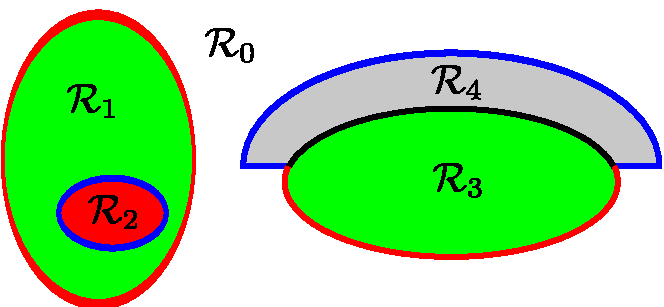
\includegraphics{RegionsAndSurfaces1.pdf}}
\caption{Schematic depiction of a {\sc scuff-em} geometry containing
         nested surfaces and three-material junctions.
         The body at left is a silicon ellipsoid ($\mc R_1$)
         that fully contains an SiO$_2$ subregion ($\mc R_2$).
         The object at right is a silicon ellipsoid partially
         coated with gold; the interior of the ellipsoid and 
         the interior of the gold coating layer are regions 
         $\mc R_3$ and $\mc R_4$ respectively.
         }
\label{RegionsAndSurfaces1}
\vspace{1in}
\resizebox{\textwidth}{!}{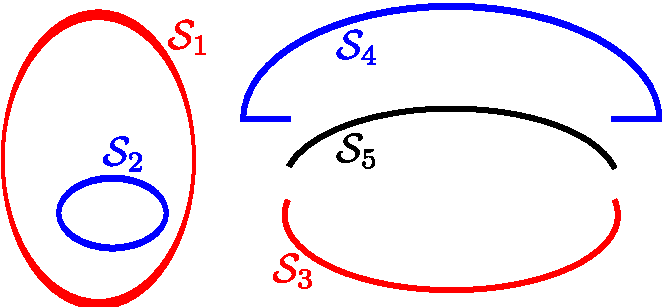
\includegraphics{RegionsAndSurfaces2.pdf}}
\caption{The surfaces for the geometry of 
         Figure \ref{RegionsAndSurfaces1}. Regions $\mc R_1$
         and $\mc R_2$ are bounded by the closed surfaces
         $\mc S_1$ and $\mc S_2$, while regions $\mc R_3$ and
         $\mc R_4$ are bounded by appropriate unions of the 
         open surfaces $\mc S_3, \mc S_4, \mc S_5.$
         More specifically, the region boundaries are 
         $ \partial R_1=S_1,
            \partial R_2=S_2,
            \partial R_3=\mc S_3 \cup \mc S_5, 
            \partial R_4=\mc S_4 \cup \mc S_5.
         $
         }
\label{RegionsAndSurfaces2}
\end{center}
\end{figure}
%####################################################################%

\begin{figure}
\begin{center}
\begin{verbcode}
  REGION R3 MATERIAL Silicon
  REGION R4 MATERIAL Gold

  OBJECT  S1 
	MESHFILE S1.msh
	MATERIAL Silicon
  ENDOBJECT

  OBJECT  S2 
	MESHFILE S2.msh
	MATERIAL SiO2
  ENDOBJECT

  SURFACE S3
        MESHFILE S3.msh
        REGIONS EXTERIOR R3
  ENDSURFACE

  SURFACE S4
        MESHFILE S4.msh
        REGIONS EXTERIOR R4
  ENDSURFACE

  SURFACE S5
        MESHFILE S5.msh
        REGIONS R3 R4
  ENDSURFACE
\end{verbcode}
\end{center}
\caption{Sample \texttt{.scuffgeo} file for the geometry 
         of Figure \ref{RegionsAndSurfaces1}.}
\label{scuffgeoFile}
\end{figure}
%####################################################################%

%%%%%%%%%%%%%%%%%%%%%%%%%%%%%%%%%%%%%%%%%%%%%%%%%%%%%%%%%%%%%%%%%%%%%%
%%%%%%%%%%%%%%%%%%%%%%%%%%%%%%%%%%%%%%%%%%%%%%%%%%%%%%%%%%%%%%%%%%%%%%
%%%%%%%%%%%%%%%%%%%%%%%%%%%%%%%%%%%%%%%%%%%%%%%%%%%%%%%%%%%%%%%%%%%%%%
\subsection*{Energy and momentum flux from field bilinears}

The Poynting flux and Maxwell stress tensor are quadratic functions
of the field components and may be conveniently written in the form
of 6-dimensional vector-matrix-vector products. 
In particular, the power flux in the direction of a unit vector 
$\vbhat{n}$ is
%====================================================================%
\begin{align}
 \vb P(\vb x) \cdot \vbhat{n}
   &=\frac{1}{2}\text{ Re }\varepsilon_{ijk}\vbhat{n}_i E^*_j(\vb x) H_k(\vb x)
\nn
   &=\frac{1}{4}\bmc{F}^\dagger(\vb x) \, \bmc{N}\supt{P}(\vbhat{n}) \, \bmc{F}(\vb x)
\label{PVMVP}
\end{align}
%====================================================================%
with
%====================================================================%
$$
   \bmc N\supt{P}=
   \left(\begin{array}{cc}
   0       & \vb N\supt{P}   \\ [3pt]
  -\vb N\supt{P} & 0
   \end{array}\right), 
\qquad 
   \vb N\supt{P}
   =
   \left(\begin{array}{ccc}
   0          &  \hat{n}_z & -\hat{n_y} \\
  -\hat{n}_z  &  0         & +\hat{n_x} \\
   \hat{n}_y  & -\hat{n}_x & 0
   \end{array}\right).
$$
%====================================================================%
Similarly, the flux of $\vbhat{u}$-directed linear momentum is
%--------------------------------------------------------------------%
\begin{align}
 \vbhat{u} \cdot \vb T(\vb x) \cdot \vbhat{n} 
&=\frac{1}{2}\text{ Re } u_i
  \left[ \epsilon E^*_i(\vb x) E_j(\vb x) 
             +\mu H^*_i(\vb x) H_j(\vb x) 
       -\frac{\delta_{ij}}{2}
         \Big( \epsilon |\vb E|^2
              +\mu      |\vb H|^2
         \Big)
 \right] \hat {n}_j
\nn
&= \frac{1}{4}\bmc{F}^\dagger(\vb x) 
   \, \bmc{N}\supt{F} \, \bmc{F}(\vb x)
\label{IFVMVP}
\end{align}
with
%--------------------------------------------------------------------%
$$
   \bmc N\supt{F}
    =
   \left(\begin{array}{cc}
   \epsilon \vb N\supt{F} & 0 \\
            0        & \mu \vb N\supt{F}
   \end{array}\right)
$$
%--------------------------------------------------------------------%
where the $3\times 3$ matrix $\vb N\supt{F}$ 
involves the outer product
of $\vbhat{u}$ and $\vbhat{n}$:
%--------------------------------------------------------------------%
$$ \vb N\supt{F}(\vbhat{u}, \vbhat{n})
   =  \vbhat{u} \vbhat{n}^T
     +\vbhat{n} \vbhat{u}^T
     +(\vbhat{u} \cdot \vbhat{n})\vb 1
$$
or
$$ N\supt{F}_{ab}(\vbhat{u}, \vbhat{n}) =
   \hat{u}_{a} \hat{n}_b + \hat{n}_a \hat{u}_b 
  - (\vbhat{u} \cdot \vbhat{n})\delta_{ab}.
$$
%====================================================================%
For example, if we are computing the $x$-force ($\vbhat{u}=\vbhat{x}$)
we have 
%====================================================================%
$$ \vb N\supt{F}(\vbhat{x}, \vbhat{n})=
   \left(\begin{array}{ccc}
   \hat{n}_x & \hat n_y   & \hat n_z \\
   \hat{n}_y & -\hat{n}_x & 0 \\
   \hat{n}_z & 0          & -\hat{n}_x
  \end{array}\right).
$$
The flux of $\vbhat{u}$-directed \textit{angular} momentum, useful
for computations of torque about an origin $\vb x_0$, is
%====================================================================%
\begin{align}
 \vbhat{u} \cdot \Big[ (\vb x-\vb x_0) \times \vb T \Big]
 \cdot \vbhat{n}
&=\frac{1}{2}
  \text{ Re }
  \hat{u}_i
  \varepsilon_{ijk}(\vb x-\vb x_0)_j T_{k\ell}(\vb x) \hat{n}_\ell
\\
&= \frac{1}{4}\bmc{F}^\dagger(\vb x) 
   \, \bmc{N}\supt{T} \, \bmc{F}(\vb x)
\label{ITVMVP}
\end{align}
%====================================================================%
with 
%--------------------------------------------------------------------%
$$
   \bmc N\supt{T}=
   \left(\begin{array}{cc}
   \epsilon \vb N\supt{T} & 0 \\
            0        & \mu \vb N\supt{T} 
   \end{array}\right)
$$
%--------------------------------------------------------------------%
where the $3\times 3$ matrix $N\supt{T}$ has entries ($\vb D=\vb x-\vb x_0$)
%--------------------------------------------------------------------%
$$ N\supt{T}_{ab}(\vbhat{u}, \vbhat{n})=
   \varepsilon_{ija}\hat{u}_i D_j \hat{n}_b
  +\varepsilon_{ijb}\hat{u}_i D_j \hat{n}_a
  -\delta_{ab} \varepsilon_{ijk} \hat{u}_i D_j \hat{n}_k.
$$

%%%%%%%%%%%%%%%%%%%%%%%%%%%%%%%%%%%%%%%%%%%%%%%%%%%%%%%%%%%%%%%%%%%%%%
%%%%%%%%%%%%%%%%%%%%%%%%%%%%%%%%%%%%%%%%%%%%%%%%%%%%%%%%%%%%%%%%%%%%%%
%%%%%%%%%%%%%%%%%%%%%%%%%%%%%%%%%%%%%%%%%%%%%%%%%%%%%%%%%%%%%%%%%%%%%%
\subsection*{Energy and momentum flux from surface-current bilinears}

Equations (\ref{PVMVP}), (\ref{IFVMVP}), and (\ref{ITVMVP}) express
the flux of power or momentum as bilinear products of the field
six-vectors $\bmc F$. Using (\ref{FFromC}), we can turn these into
bilinear products of the surface-current coefficient vectors
$\vb c$. For example, the power flux in the $\vbhat{n}$
direction, equation (\ref{PVMVP}), becomes 
%--------------------------------------------------------------------%
\begin{align}
 \vb P(\vb x) \cdot \vbhat{n}
&=\frac{1}{4}\bmc F^\dagger(\vb x) \bmc N\supt{P}(\vbhat{n}) \bmc F(\vb x)
\nn
&=\frac{1}{4}\sum_{\alpha \beta} 
  c_\alpha^* 
  \Big[ \bmc F^\dagger_\alpha(\vb x)
        \,
        \bmc N\supt{P}(\vbhat{n})
        \,
        \bmc F_\beta(\vb x)
  \Big]
  c_\beta 
\label{PFluxSum}\\
&= \vb c^\dagger \vb Q\supt{PFLUX}(\vbhat{n}, \vb x) \vb c 
\label{PFluxVMVP}
\end{align}
%--------------------------------------------------------------------%
where $\vb Q\supt{PFLUX}(\vbhat{n}, \vb x)$ is a matrix 
appropriate for $\vbhat{n}$-directed power flux at $\vb x$.
[As in equation (\ref{FFromCProper}), the sum over 
 $\alpha,\beta$ in (\ref{PFluxSum}) runs only over basis 
 functions lying on the boundary of the region
 containing the evaluation point $\vb x$.]
The fluxes of $\vbhat{u}$-directed linear and angular 
momentum read similarly
%--------------------------------------------------------------------%
\begin{align}
\vbhat{u} \cdot \vb T(\vb x) \cdot \vbhat{n}
&= \vb c^\dagger \vb Q\supt{FFLUX}(\vbhat{u}, \vbhat{n}, \vb x) \vb c
\label{IFFluxVMVP}
\\
\vbhat{u} 
 \cdot \Big[ (\vb x-\vb x_0) \times \vb T(\vb x) \Big]
 \cdot \vbhat{n}
&= \vb c^\dagger \vb Q\supt{TFLUX}(\vbhat{u}, \vbhat{n}, \vb x) \vb c
\label{ITFluxVMVP}
\end{align}
%--------------------------------------------------------------------%
The $\vb Q$ matrices in (\ref{PFluxVMVP}), (\ref{IFFluxVMVP}), and 
(\ref{ITFluxVMVP}) are $N\subt{B}\times N\subt{B}$ matrices
whose entries are themselves 6-dimensional matrix-vector products:
%====================================================================%
\begin{subequations}
\begin{align}
Q_{\alpha\beta}\supt{PFLUX}(\vbhat{n}, \vb x)
 &= \frac{1}{4} 
    \bmc F^\dagger_\alpha(\vb x) 
    \bmc N\supt{P}(\vbhat{n}, \vb x)
    \bmc F_\beta(\vb x) 
\\
Q_{\alpha\beta}\supt{FFLUX}(\vbhat{u}, \vbhat{n}, \vb x)
 &= \frac{1}{4} 
    \bmc F^\dagger_\alpha(\vb x) 
    \bmc N\supt{F}(\vbhat{u}, \vbhat{n}, \vb x)
    \bmc F_\beta(\vb x) 
\\
Q_{\alpha\beta}\supt{TFLUX}(\vbhat{u}, \vbhat{n}, \vb x)
 &= \frac{1}{4} 
    \bmc F^\dagger_\alpha(\vb x) 
    \bmc N\supt{T}(\vbhat{u}, \vbhat{n}, \vb x)
    \bmc F_\beta(\vb x).
\end{align}
\label{SixBySixVMVPs}
\end{subequations}
%====================================================================%

%%%%%%%%%%%%%%%%%%%%%%%%%%%%%%%%%%%%%%%%%%%%%%%%%%%%%%%%%%%%%%%%%%%%%%
%%%%%%%%%%%%%%%%%%%%%%%%%%%%%%%%%%%%%%%%%%%%%%%%%%%%%%%%%%%%%%%%%%%%%%
%%%%%%%%%%%%%%%%%%%%%%%%%%%%%%%%%%%%%%%%%%%%%%%%%%%%%%%%%%%%%%%%%%%%%%
\subsection*{Power, force, and torque from surface-current bilinears}

The main quantities of interest in {\sc scuff-neq} are the
power, force, or torque (PFT) on individual bodies in a geometry.
There are actually three separate ways to derive surface-current 
bilinear expressions for these quantities, which we here consider 
in turn.

\subsubsection*{Dense surface-integral PFT bilinears}

The simplest way to obtain surface-current bilinears for the
total PFT on one or more bodies is simply to integrate the 
spatially-resolved fluxes of the previous section over a closed
bounding surface $\mc S$ containing the bodies.
Indeed, noting that the $\vb x$ and $\vbhat{n}$ dependence of
the flux expressions (\ref{PFluxVMVP}), (\ref{IFFluxVMVP}),
and (\ref{ITFluxVMVP}) is entirely contained in the $\vb Q$
matrices, it is easy to integrate those expressions over
$\mc S$, then pull the surface-current vectors $\vb c$
outside the integral to identify what we shall call
the \textit{displaced surface-integral PFT} (DSIPFT) matrices. 

For example, the total power absorbed by material bodies
contained within a closed surface $\mc S$
is given by integrating the LHS of (\ref{PFluxVMVP})
over $\mc S$:
%====================================================================%
\begin{align}
  P_{\mc S}\sups{abs}&=\int_{\mc S} \vb P(\vb x) \cdot \vbhat{n} \, d\vb x
\intertext{with $\vbhat{n}$ taken to be the inward-pointing surface
           normal. Insert the RHS of (\ref{PFluxVMVP}) and pull 
           $\vb c^\dagger, \vb c$ outside the integral:}
             &=\vb c^\dagger \vb Q\supt{PTOT} \vb c
\label{PTotVMVP}
\end{align}
where the elements of 
$\vb Q\supt{PTOT}$
involve integrals over $\mc S$:
%====================================================================%
\begin{align}
Q_{\alpha\beta}\supt{PTOT}(\mc S)
  &= \frac{1}{4} \int_{\mc S}
    \bmc F^\dagger_\alpha(\vb x)
    \bmc N\supt{P}(\vbhat{n})
    \bmc F_\beta(\vb x)
     \, d\vb x
\intertext{If $\{w_p, \vb x_p\}$ is an $N\subt{C}$-point
           cubature rule for integrating over $\mc S$, this may
           be approximated as}
  &\approx \frac{1}{4} \sum_{p=1}^{N\supt{C}} w_p
    \bmc F^\dagger_\alpha(\vb x_p)
    \bmc N\supt{P}(\vbhat{n}_p)
    \bmc F_\beta(\vb x_p)
\label{QPTOTEntries}
\end{align}
%====================================================================%
where $\vbhat{n}_p$ is the normal to $\mc S$ at $\vb x_p.$
%====================================================================%
Similarly, the time-average $\vbhat{u}$-directed force and 
torque on material bodies contained in $\mc S$ are
%====================================================================%
\begin{align}
 F_{\mc S}(\vbhat{u}) &=\vb c^\dagger \vb Q\supt{FTOT}\vb c
\label{FTotVMVP}
\\
 \mc T_{\mc S}(\vbhat{u}) &=\vb c^\dagger \vb Q\supt{TTOT}\vb c
\label{TTotVMVP}
\end{align}
%====================================================================%
where the entries of $\vb Q\supt{FTOT}$ and $\vb Q\supt{TTOT}$ 
are similar to (\ref{QPTOTEntries}) with 
$\bmc N\supt{P} \to \bmc N\supt{F}, \bmc N\supt{T}.$

%%%%%%%%%%%%%%%%%%%%%%%%%%%%%%%%%%%%%%%%%%%%%%%%%%%%%%%%%%%%%%%%%%%%%%
%%%%%%%%%%%%%%%%%%%%%%%%%%%%%%%%%%%%%%%%%%%%%%%%%%%%%%%%%%%%%%%%%%%%%%
%%%%%%%%%%%%%%%%%%%%%%%%%%%%%%%%%%%%%%%%%%%%%%%%%%%%%%%%%%%%%%%%%%%%%%
\subsubsection*{Other $\vb Q$ matrices for spatially-integrated PFTs}

For some quantities of interest it is possible to write alternative
surface-current bilinears that compute the same quantities as 
(\ref{PTotVMVP}), (\ref{FTotVMVP}), and (\ref{TTotVMVP})
using different matrices. This is discussed 
in \citeasnoun{Reid2013a}.

\subsubsection*{Simplification of $6\times 6$ matrix-vector
                products}

The preceding derivation was agnostic regarding the
choice of basis functions $\bmc B_\alpha$. For the
particular basis functions used in {\sc scuff-em},
we can write slightly more explicit expressions
for the matrix entries in equation (\ref{SixBySixVMVPs}).

In {\sc scuff-em}, each internal edge on a meshed
surface of dielectric interface corresponds
to a single RWG basis function and two surface-current
coefficients, one for electric surface current and one 
for magnetic surface current. If the edge index is $a$, 
then the RWG function is $\vb b_a(\vb x)$ and the 
electric and magnetic basis function indices are 
$\alpha=\{2a, 2a+1\}$. 

Then $\bmc F_{2a}$ and $\bmc F_{2a+1}$ in equation
(\ref{SixBySixVMVPs}) are the six-vector fields
due respectively to unit-strength electric and magnetic 
surface currents in region $\mc R_i$ (the region
containing the evaluation point):
%%====================================================================%
\begin{align*}
  \bmc F_{2a}(\vb x)
  = \left( \begin{array}{c}
    ikZ \vb e_a(\vb x) \\ \vb h_a(\vb x)
    \end{array}\right), 
\qquad
  \bmc F_{2a+1} 
 = \left( \begin{array}{c}
    -\vb h_a(\vb x) \\ \frac{ik}{Z} \vb e_a(\vb x)
    \end{array}\right)
\end{align*}
%%====================================================================%
Here $k$ and $Z$ are the wavenumber and (absolute) 
wave impedance in region $\mc R_i$ and $\vb e_a$ and $\vb h_a$
are the ``reduced fields'' due to basis function $\vb b_a$:
%%====================================================================%
$$ \vb e_a(\vb x) 
   =
   \int_{\sup \vb b_a} \vb G(k; \vb x, \vb x^\prime) 
                       \cdot \vb b_a (\vb x^\prime) 
   \, d\vb x^\prime,
   \quad
   \vb h_a(\vb x) 
   =
   -ik\int_{\sup \vb b_a} \vb C(k; \vb x, \vb x^\prime) 
                       \cdot \vb b_a (\vb x^\prime) 
   \, d\vb x^\prime.
$$
%%====================================================================%
Power flux at $\vb x$:
%%====================================================================%
\begin{align*}
 P_i(\vb x) 
&= 
 \frac{1}{2}\epsilon_{ijk}\text{Re }\Big[ E^*_j(\vb x) H_k(\vb x) \Big]
\\
&= 
 \frac{1}{4}\epsilon_{ijk}
 \Big[ E^*_j(\vb x) H_k(\vb x) + E_j(\vb x) H^*_k(\vb x) \Big]
\\
&=
 \frac{1}{4}\epsilon_{ijk}
 \Big[ E^*_j(\vb x) H_k(\vb x) - H^*_j(\vb x) E_k(\vb x) \Big]
\\
&=
 \frac{1}{4}\epsilon_{ijk}\sum_{\alpha\beta}
  \bigg\{ 
   \Big( k_\alpha \cdot ikZ \vb e_\alpha - n_\alpha \vb h_\alpha\Big)^*_j
   \Big( k_\beta \vb h_\beta             + n_\beta \cdot \frac{ik}{Z} \vb h_\beta\Big)_k
\\
&\hspace{0.7in}
  -
   \Big( k_\alpha \vb h_\alpha           + n_\alpha \cdot \frac{ik}{Z} \vb h_\alpha\Big)^*_j
   \Big( k_\beta \cdot ikZ \vb e_\alpha - n_\alpha \vb h_\alpha\Big)_k
  \bigg\}
\end{align*}

%%====================================================================%
The contributions of a single pair of basis functions
$\vb b_a, \vb b_b$ to the power and momentum flux
at $\vb x$ are
%====================================================================%
\begin{align}
 \Delta P_i
 &= \frac{1}{2}\text{Re }
    \vbhat{n}_i
    \cdot 
    \Big(ikZ k_\alpha \vb e_\alpha - n_\alpha \vb h_\alpha\Big)^* 
    \times
    \Big( k_\beta \vb h_\beta + \frac{ik}{Z} n_\beta \vb e_\beta \Big)
\\
&= \frac{1}{2}\text{Re }
   \left(\begin{array}{c}
     k_\alpha \\ n_\alpha 
   \end{array}\right)^\dagger
   \left(\begin{array}{cc}
    (ikZ)^*              \vb e^*_\alpha \times \vb h_\beta & 
    |k|^2 \frac{Z^*}{Z}  \vb e^*_\alpha \times \vb e_\beta \\
  -                      \vb h^*_\alpha \times \vb h_\beta & 
  - \frac{ik}{Z}         \vb h^*_\alpha \times \vb e_\beta
   \end{array}\right)
   \left(\begin{array}{c}
     k_\beta\\ n_\beta
   \end{array}\right)
\\
 \Delta T_{ij}
 &= \frac{1}{2}\text{Re }
    \left(\begin{array}{c}
    ikZ k_\alpha \vb e_\alpha - n_\alpha \vb h_\alpha \\
        k_\alpha \vb h_\alpha + \frac{ik}{Z} n_\alpha \vb e_\alpha
    \end{array}\right)
\end{align}

%====================================================================%
%====================================================================%
%====================================================================%
\newpage
\bibliographystyle{ieeetr}
\bibliography{scuff-neq}

\end{document}
